\chapter{Learning Paradigms}\label{ch:para}

Throughout this thesis, we assume to be given data $\domain_n\subset\domain\subset \R^d$ consisting of $n$ data points. We consider task of \emph{learning} a function $u:\tilde{\domain}\to \Upsilon$ from the given data, where the two most important cases for us are
%
\begin{itemize}
\item \textbf{classification}: $u$ assigns a label to each $x\in D$ out of a total of $C\in\N$ possible classes, i.e. $\Upsilon=\{1,\ldots,C\}$.
%
\item \textbf{image denoising}: $u$ outputs a denoised version of an input image $x$, i.e. here $\tilde{\domain} = \Upsilon$.
\end{itemize}
%
The set $\tilde{\domain}\subset\R^d$ is usually either the set of data points $\domain_n$ or the whole space $\domain$. The learning paradigms we consider in this thesis, differ by their use of labeled data. We review the concepts in the following.
%
\section{Unsupervised Learning}
\begin{wrapfigure}{r}{.5\textwidth}
\centering
\includegraphics[width=.5\textwidth]{atelier/paradigms/UL.pdf}
\end{wrapfigure}

In this case we are not given any labeled data. In our context the most important application is data clustering. Other tasks involve dimensionality reduction or density estimation, see \cite{subramanya2014graph}. The clustering task consists of grouping data based on some similarity criterion. In this sense, clustering can also be interpreted as classification, i.e., the desired function is a mapping $u:\tilde{\domain}\to \{1,\ldots, C\}$ where $C\in\N$ denotes the number of clusters. Typically, one wants to obtain a clustering of the given data set, i.e., $\mathcal{\domain} = \domain$. We list some of the typical clustering methods below.
%
\begin{itemize}
\item K-means algorithm, \cite{steinhaus1956division},
\item Expectation Maximization, \cite{dempster1977maximum},
\item Cheeger cuts, \cite{GarcSlep15, szlam2009total, trillos2016consistency, garcia2022graph},
\item spectral clustering, \cite{trillos2018variational}.
\end{itemize}
%
%
Unsupervised learning is not the main focus of this present work. However, we note that especially the concepts developed in \cite{GarcSlep15} for Cheeger cuts are crucial for the continuum limit framework in \cref{sec:GConv}.

\section{Supervised Learning}\label{sec:PSL}
\begin{wrapfigure}{r}{.5\textwidth}
\centering
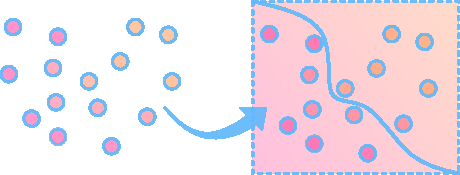
\includegraphics[width=.5\textwidth]{atelier/paradigms/SL.pdf}
\end{wrapfigure}
%
In this setting, each data point $x\in\domain_n$ is labeled, via a given function $g:\domain_n\to\Upsilon$ such that we have a finite training set $\mathcal{T} = \{(x,g(x)): x\in\domain_n\}$. The task is then to infer a function defined on the underlying space, i.e. $u:\domain \to\Upsilon$, i.e. we want to assign a label to unseen $x\in\domain$ that are not necessarily part of the given data. In order to \emph{learn} the function $u$ from the given data, one needs to choose a parameterized class of functions $\mathcal{U}$, where typically each element can be describe by a finite number of parameters. Among others, common methods or parametrizations include
%
\begin{itemize}
\item Support vector machines \cite{cortes1995support, scholkopf2005support},
\item decision Trees \cite{morgan1963problems, Brei},
\item neural networks \cite{Turing,rosenblatt1958perceptron, minsky1969introduction}.
\end{itemize}
%
In \cref{sec:SL} we exclusively focus on supervised learning algorithms employing neural networks. We refer to \cite{SCHMIDHUBER201585} for an exhaustive historical overview. The concrete setting and learning framework is given in \cref{sec:SL}.
%
%
%
\section{Semi-Supervised Learning}\label{sec:PSSL}
\begin{wrapfigure}{r}{.5\textwidth}
\centering
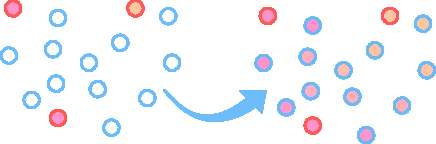
\includegraphics[width=.5\textwidth]{atelier/paradigms/SSL.pdf}
\end{wrapfigure}
%
In the semi-supervised setting we assume that only a fraction of the data $\domain_n$ is labeled, i.e., we are given a a function $g:\conset_n\to\Upsilon$ where $\conset_n\subset\domain_n$ is the set of labeled data. Typically the labeled data constitutes only a small fraction of all available points, i.e. $\abs{\conset_n}<<\abs{\domain_n}$. In this thesis we restrict ourselves to the \emph{transductive setting}, i.e. we ant to infer a function acting only on the data $u: \domain_n\to \Upsilon$. This is opposed to the inductive setting, where $u$ also classifies unseen points $x\in\domain$, \cite{zhu2005semi}. Common algorithms and methods include
%
\begin{itemize}
\item expectation maximization and mixture models \cite{??},
\item self-training and co-training \cite{??},
\item graph-based learning \cite{zhu2005semi}.
\end{itemize}
%
%
In \cref{ch:SSL} we focus on graph-based learning algorithms, however we refer to \cite{zhu2005semi} for a wonderful overview of semi-supervised learning algorithms.